\documentclass[12pt,a4paper]{ctexart}

% ============================================================
% 格式对齐 docs/格点QCD中的** 系列
% 编译：XeLaTeX 两遍
% ============================================================
\usepackage[top=2.5cm,bottom=2.5cm,left=2.5cm,right=2.5cm]{geometry}
\usepackage{amsmath,amssymb,amsthm}
\usepackage{physics}
\usepackage{graphicx,float,booktabs,array,caption,multirow}
\usepackage{hyperref,xcolor,enumitem,mathtools}
\usepackage[numbers,sort&compress]{natbib}
\usepackage{tabularx,xltabular}
\usepackage{seqsplit}
\usepackage{tikz}
\usetikzlibrary{arrows.meta,positioning,calc,decorations.markings}

\hypersetup{colorlinks=true,linkcolor=blue,citecolor=blue,urlcolor=blue}
\urlstyle{same}
\theoremstyle{definition}
\newtheorem{definition}{定义}[section]
\newtheorem{remark}{注记}[section]
\newtheorem{theorem}{定理}[section]

\setlength{\emergencystretch}{2.5em}
\allowdisplaybreaks

\newcommand{\MSbar}{\overline{\mathrm{MS}}}
\newcommand{\ii}{\mathrm{i}}
\newcommand{\ee}{\mathrm{e}}
\newcommand{\Pplus}{P^+}
\newcommand{\qgpd}{\widetilde H}
\renewcommand{\path}[1]{\seqsplit{\textsf{\detokenize{#1}}}}
\newcommand{\GPD}{\mathrm{GPD}}

\tikzset{
  quark/.style={
    postaction={decorate},
    decoration={markings,
      mark=at position 0.55 with {\arrow{>}}},
    line width=0.8pt
  }
}

\title{\heiti 格点QCD中的广义部分子分布：\\
从光锥矩阵元、准GPD到非前行匹配}
\author{基于本库全部相关文献、论文与代码的综合解析}
\date{\today}

\begin{document}

\maketitle

\begin{abstract}
\noindent
广义部分子分布（Generalized Parton Distributions, GPDs）是部分子分布函数（PDFs）
在非前行（off-forward）运动学下的推广。PDF 只回答“强子中纵向动量份额为 $x$ 的
部分子有多少”，而 GPD 同时编码初末强子动量差 $\Delta=P_f-P_i$ 与纵向斜度
$\xi$，并把一维纵向图像扩展到横向位置空间。它与深度虚 Compton 散射（DVCS）、
深度虚介子产生（DVMP）、核子形状因子、自旋角动量分解、横向位置层析以及 TMD/PDF
的关联处在同一理论网络中。

本文面向“格点 QCD 中如何理解并计算 GPD”这一主题，按照本库
“格点QCD中的”系列文档的章节深度组织材料。正文从光锥算符和
$x,\xi,t$ 运动学出发，系统给出夸克与胶子 GPD 的定义、Lorentz 分解、
DGLAP/ERBL 支撑区、前向与形状因子极限、多项式性、双分布表示、正定性、
冲击参数层析和 Ji 角动量求和规则；随后讨论 Euclidean 三点函数、
Wilson 线、非前行动量、比值提取、非微扰重整化、准 GPD/伪 GPD 的双 Fourier
变换及夸克--胶子 NLO 匹配矩阵。最后单独核对本库生产代码：截至本文审计版本，
\texttt{pyqcd/} 已具备任意动量相位、非局域胶子算符、VdV/VVV、自动 Wick、
三个月点比值等可复用基元，但尚无 GPD 专用生产链或真实数据验证。

本文严格区分四种状态：\textbf{理论定义成立}、\textbf{受控测试通过}、
\textbf{格点算符或算法存在}、\textbf{真实 GPD 数值已闭合}。四者不能互相替代。
\end{abstract}

\tableofcontents
\newpage

%==========================================================================
\section{引言：为什么需要 GPD}
%==========================================================================

\subsection{从一维 PDF 到非前行矩阵元}

共线 PDF 描述强子在一个特定 Fock 态中找到一个携带纵向动量份额 $x$ 的部分子的
概率密度。其常见光锥定义包含强子--强子矩阵元，但初末强子态具有相同动量：
\begin{equation}
q(x,\mu)
=\int\frac{\dd z^-}{4\pi}\ee^{\ii xP^+z^-}
\langle P|\bar\psi(0)\gamma^+
W(0,z^-)\psi(z^-)|P\rangle .
\label{eq:pdf-lightcone}
\end{equation}
PDF 的概率解释和因子化成功使其成为高能散射的核心非微扰输入，但它只给出
纵向一维信息。

GPD 保留同一非局域部分子算符，却把它夹在动量不同的初末强子态之间。因此，
除 $x$ 外，还出现两个新的独立运动学变量：
\begin{itemize}[leftmargin=*]
  \item $\xi$：纵向斜度，描述初末强子纵向动量差相对于平均动量的大小；
  \item $t=\Delta^2$：动量转移平方，其 Fourier 共轭与横向位置信息相联系。
\end{itemize}

从物理图像看，PDF 是 GPD 在 $\Delta=0$ 时的对角切片；弹性形状因子是 GPD
对 $x$ 的积分；自旋角动量则可从 GPD 的一阶 Mellin 矩读出。GPD 因而位于
“部分子分布”与“强子形状/自旋结构”之间的交叉点。

\subsection{GPD 连接的主要物理对象}

\begin{table}[H]
\centering
\small
\caption{GPD 在强子结构理论网络中的位置}
\label{tab:gpd-network}
\begin{tabularx}{\textwidth}{lX}
\toprule
物理对象 & 与 GPD 的关系 \\
\midrule
PDF & $H^q(x,0,0)$ 回到夸克的非极化 PDF；$\widetilde H^q$ 回到螺旋度分布 \\
形状因子 & $\int \dd x\,H^q(x,\xi,t)=F_1^q(t)$，
$\int \dd x\,E^q(x,\xi,t)=F_2^q(t)$ \\
Ji 角动量 & $J_q=\frac12\int_{-1}^{1}\dd x\,x[H^q(x,\xi,0)+E^q(x,\xi,0)]$ \\
DVCS/DVMP & 实验通过 Compton 振幅或专属介子产生振幅对 GPD 卷积进行约束 \\
横向位置层析 & 对 $\Delta_\perp$ 作二维 Fourier 变换得到 $x$--$b_\perp$ 分布 \\
双分布 & GPD 的 Mellin 矩多项式性可由双分布表示自然保证 \\
TMD & GPD 与 TMD 通过横向位置/横向动量 Fourier 变换及软、演化因子相关联 \\
核子自旋 & $E$ 项携带自旋翻转信息，进入角动量分解与反常磁矩约束 \\
\bottomrule
\end{tabularx}
\end{table}

\subsection{格点计算的根本困难}

式~\eqref{eq:pdf-lightcone} 的分离方向 $z^-$ 是光锥方向。格点 QCD 在
Euclidean 时空中定义，Monte Carlo 权重由 $e^{-S_E}$ 给出，不能直接计算实时间
或光锥关联函数。GPD 比 PDF 还多出非前行动量与自旋投影，因此需要同时解决：
\begin{enumerate}[leftmargin=*]
  \item 用空间分离 $z$ 和 Wilson 线构造 Euclidean 准部分子算符；
  \item 分别在源、插入和汇处处理 $P_i,P_f$；
  \item 从多个 Dirac/自旋投影中分离 $H,E,\widetilde H,\widetilde E$；
  \item 消除 Wilson 线线性发散并完成与光锥 GPD 的匹配；
  \item 控制激发态、有限体积、有限格距、有限大动量和 Fourier 截断系统误差。
\end{enumerate}

本库现有的前向 PDF、TMD 和三点函数实现能覆盖其中的若干基元，但 GPD 的
“非前行运动学 + 多投影分解 + 非前行匹配”不能由其中任一单项自动得到。

\subsection{本文取证原则}

本文采用“全库索引 + 主题精读”的方式：先对 \path{docs/*.tex}、
\path{refer/papers}、\path{refer/zengch}、\path{refer/huangcl}、
\path{refer/git-rep/lamet-agent} 与 \path{pyqcd/} 搜索 GPD、non-forward、
off-forward、skewness、Wilson line、三点函数和匹配核关键词，再对定义链与代码接口
逐项核对。任何“本库已实现”的陈述都以源码或测试为证据；标准场论公式则引用
本库论文与教材，并与参考论文的定义逐项对齐。

%==========================================================================
\section{运动学、光锥算符与 GPD 定义}
%==========================================================================

\subsection{光锥坐标和符号约定}

采用
\begin{equation}
v^\pm=\frac{v^0\pm v^3}{\sqrt2},\qquad
v=(v^+,v^-,v_\perp),\qquad
v\cdot w=v^+w^-+v^-w^+-v_\perp\cdot w_\perp .
\label{eq:lightcone-convention}
\end{equation}
部分子光锥方向的分离记作 $z^-$。本文固定一个全局符号约定：初始强子动量为
$P_i$，末态强子动量为 $P_f$，并定义
\begin{equation}
P=\frac{P_i+P_f}{2},\qquad
\Delta=P_f-P_i,\qquad
t=\Delta^2,\qquad
\xi=\frac{P_i^+-P_f^+}{P_i^++P_f^+}
=-\frac{\Delta^+}{2P^+}.
\label{eq:gpd-kinematics}
\end{equation}
于是 $P_i=P-\Delta/2$、$P_f=P+\Delta/2$。大动量计算通常取
$P^z$ 很大，而 $\Delta_\perp$ 提供空间横向动量转移；不指定全局符号时，
$\xi$、Fourier 相位和 $E$ 项很容易出现无法追踪的整体换号。

GPD 的物理支撑区为
\begin{equation}
x\in[-1,1],\qquad |\xi|\leq 1 .
\label{eq:gpd-support}
\end{equation}
其中 $|x|>|\xi|$ 称为 DGLAP 区，$|x|<|\xi|$ 称为 ERBL 区。前者在
$\xi\to0$ 时连续退化为普通 PDF/反夸克分布；后者描述夸克--反夸克振幅，
不能把它直接解释为“反夸克概率密度”。

\begin{figure}[H]
\centering
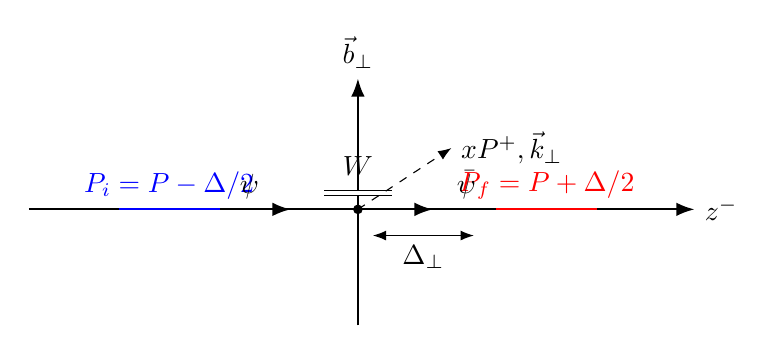
\begin{tikzpicture}[scale=0.95,>=Latex]
  \draw[->,thick] (-4.4,0) -- (4.5,0) node[right] {$z^-$};
  \draw[->,thick] (0,-1.55) -- (0,1.75) node[above] {$\vec b_\perp$};
  \draw[thick,blue] (-3.2,0) -- (-1.85,0) node[midway,above] {$P_i=P-\Delta/2$};
  \draw[thick,red] (1.85,0) -- (3.2,0) node[midway,above] {$P_f=P+\Delta/2$};
  \draw[quark] (-1.45,0) node[above] {$\psi$} -- (-0.45,0);
  \draw[quark] (0.45,0) -- (1.45,0) node[above] {$\bar\psi$};
  \draw[double,double distance=1.5pt] (-0.45,0.22) -- (0.45,0.22);
  \node at (0,0.58) {$W$};
  \filldraw (0,0) circle (1.6pt);
  \draw[dashed,->] (0,0) -- (1.25,0.82) node[right] {$xP^+,\vec k_\perp$};
  \draw[<->] (0.2,-0.35) -- (1.55,-0.35) node[midway,below] {$\Delta_\perp$};
\end{tikzpicture}
\caption{GPD 的非前行运动学示意。初末强子动量相差 $\Delta$；部分子在
光锥方向携带平均纵向动量份额 $x$，横向位置与动量转移的 Fourier 共轭相联系。}
\label{fig:gpd-kinematics}
\end{figure}

\subsection{夸克双局域算符}

夸克 GPD 从基本表示中的双局域算符出发：
\begin{equation}
\begin{aligned}
\mathcal O_q^{\Gamma}(z_1,z_2)
&=\bar\psi(z_1)\Gamma[z_1,z_2]\psi(z_2),\\
[z_1,z_2]&=\mathcal P\exp\!\left[
\ii g\int_0^1\dd t\,(z_1-z_2)\cdot A(z_2+t(z_1-z_2))
\right].
\end{aligned}
\label{eq:quark-bilocal}
\end{equation}
在光锥极限取 $z_1=-z^-/2$、$z_2=z^-/2$。对称化后，核子矩阵元可写成
\begin{equation}
\begin{aligned}
&\int\frac{\dd z^-}{4\pi}\ee^{\ii xP^+z^-}
\langle P_f,S_f|
\bar\psi\!\left(-\frac{z^-}{2}\right)\gamma^+
W\!\left(-\frac{z^-}{2},\frac{z^-}{2}\right)
\psi\!\left(\frac{z^-}{2}\right)
|P_i,S_i\rangle \\
&=\bar u(P_f,S_f)\left[
\gamma^+H^q(x,\xi,t)
+\frac{\ii\sigma^{+\mu}\Delta_\mu}{2M}E^q(x,\xi,t)
\right]u(P_i,S_i).
\end{aligned}
\label{eq:vector-gpd-decomposition}
\end{equation}
轴矢通道为
\begin{equation}
\begin{aligned}
&\int\frac{\dd z^-}{4\pi}\ee^{\ii xP^+z^-}
\langle P_f,S_f|
\bar\psi\!\left(-\frac{z^-}{2}\right)\gamma^+\gamma_5
W\!\left(-\frac{z^-}{2},\frac{z^-}{2}\right)
\psi\!\left(\frac{z^-}{2}\right)
|P_i,S_i\rangle \\
&=\bar u(P_f,S_f)\left[
\gamma^+\gamma_5\widetilde H^q(x,\xi,t)
+\frac{\Delta^+}{2M}\gamma_5\widetilde E^q(x,\xi,t)
\right]u(P_i,S_i).
\end{aligned}
\label{eq:axial-gpd-decomposition}
\end{equation}
横向极化还给出张量族
$H_T^q,E_T^q,\widetilde H_T^q,\widetilde E_T^q$。其完整 Lorentz 基含有
$\sigma^{+\mu}$ 与 $\Delta^\mu$ 的不同组合，具体归一化和 $E$ 项符号必须与
所用自旋旋量约定整体固定。

\begin{remark}
式~\eqref{eq:vector-gpd-decomposition} 是本文的主约定。若论文采用
$\Delta=P_i-P_f$ 或把初态记为 $P_1$、末态记为 $P_2$，其 $\xi$、Fourier
相位以及 $H/E$ 的符号可能与本文不同。正确做法是整体重写定义并检验
$\xi=0,t=0$ 的 PDF 极限和弹性形状因子极限，而不是只给某一条公式换号。
\end{remark}

\subsection{自旋零与自旋二分之一的差别}

对无自旋强子，例如 $\pi$ 介子，矢量通道的最低阶分解不含自旋翻转项，可写为
\begin{equation}
\langle\pi(P_f)|\mathcal O_q^{\gamma^+}(-z^-/2,z^-/2)|\pi(P_i)\rangle
\simeq 2P^+H^{\pi,q}(x,\xi,t).
\label{eq:pion-gpd}
\end{equation}
自旋 $1/2$ 核子需要至少两个独立矢量结构 $H,E$，以及两个轴矢结构
$\widetilde H,\widetilde E$。这不是“多写几个函数”，而是来自旋量双线性
在 Lorentz、宇称和时间反演下的不可约分解。

在格点上，$H,E$ 不能靠单个三点函数直接读出。必须选取不同的
$\Gamma$、初末自旋投影和动量方向，构造完整的投影矩阵；随后解线性方程或
拟合矩阵元。若只有一个投影，就不能把结果同时称为 $H$ 和 $E$。

\subsection{胶子 GPD}

胶子算符含有两个场强张量，Wilson 线位于伴随表示：
\begin{equation}
\mathcal O_g^{\mu\nu,\rho\sigma}(z_1,z_2)
=F^{a,\mu\nu}(z_1)
W^{ab}_{\rm adj}(z_1,z_2)
F^{b,\rho\sigma}(z_2).
\label{eq:gluon-bilocal}
\end{equation}
非极化胶子 GPD 由横向投影组合定义，极化通道使用对偶场强
$\widetilde F^{\mu\nu}=\frac12\epsilon^{\mu\nu\rho\sigma}F_{\rho\sigma}$。
与夸克情形相比，胶子算符有三个额外复杂性：
\begin{enumerate}[leftmargin=*]
  \item 场强张量具有两个 Lorentz 指标，存在更多不可约结构；
  \item Wilson 线处于伴随表示，重整化常数依赖算符中沿 $z$ 的指标数；
  \item 胶子插入与核子之间没有价夸克线连接，三点函数天然含有非连通贡献。
\end{enumerate}

本库 \path{pyqcd/operator/_gluon_ope.py} 已实现 Clover 场强、直线/反向
Wilson 线、双场强和若干 Lorentz 对组合，可作为胶子 GPD 的几何与算符前驱；
但现有接口服务前向 OPE/TMD，尚没有非前行核子态的 GPD 契约。

\subsection{夸克与胶子 GPD 命名对照}

\begin{table}[H]
\centering
\small
\caption{核子 leading-twist GPD 的主要通道}
\label{tab:gpd-channels}
\begin{tabularx}{\textwidth}{l l l X}
\toprule
极化 & 夸克通道 & 胶子通道 & 物理内涵 \\
\midrule
非极化 & $H,E$ & $H_g,E_g$ & 动量分布与自旋翻转、角动量 \\
纵向极化 & $\widetilde H,\widetilde E$ & $\widetilde H_g,\widetilde E_g$ & 螺旋度与轴矢结构 \\
横向极化 & $H_T,E_T,\widetilde H_T,\widetilde E_T$ & 胶子横向性 & 手征奇、张量结构 \\
\bottomrule
\end{tabularx}
\end{table}

横向性夸克通道在共线因子化中与胶子不混合；非极化和螺旋度的味单态夸克通道
则可以在\emph{微扰匹配阶段}通过 $C_{qg},C_{gq}$ 与胶子 GPD 混合。
这一混合与 Wilson 线算符的 UV 乘法重整化是不同层次的问题。

%==========================================================================
\section{解析性质、物理极限与解释}
%==========================================================================

\subsection{DGLAP 区与 ERBL 区}

GPD 的 $x$ 支撑可按 $|x|$ 与 $|\xi|$ 的关系分为两区：
\begin{equation}
\text{DGLAP: } |x|\geq|\xi|,\qquad
\text{ERBL: } |x|\leq|\xi|.
\label{eq:dglap-erbl}
\end{equation}
在 DGLAP 区，夸克和反夸克可以作为概率型的部分子密度理解；在 ERBL 区，
算符连接的是夸克--反夸克对，物理上更接近分布振幅。演化方程在不同区域具有
不同的积分边界和核函数，但边界连续性由 forward-like 约束和不连续项保证。

GLAP 演化可概括为
\begin{equation}
\mu\frac{\partial}{\partial\mu}H(x,\xi,t)
=\int \dd y\,V(x,y;\xi)\,H(y,\xi,t),
\label{eq:gpd-evolution}
\end{equation}
其中当 $|x|>|\xi|$ 时核函数回到 DGLAP 型劈裂结构，当 $|x|<|\xi|$ 时进入
ERBL 型演化。完整的非前行核含 $\xi$ 依赖，不能只把前向 DGLAP 核直接代入
ERBL 区域。

\subsection{前向 PDF 极限}

当 $\Delta=0$，即 $\xi=t=0$，GPD 退化为普通 PDF：
\begin{align}
H^q(x,0,0)&=q(x),&
H^q(-x,0,0)&=-\bar q(x), \qquad x>0,\\
\widetilde H^q(x,0,0)&=\Delta q(x),&
\widetilde H^q(-x,0,0)&=\Delta\bar q(x), \qquad x>0,\\
H_T^q(x,0,0)&=\delta q(x),&
H_T^q(-x,0,0)&=-\delta\bar q(x), \qquad x>0 .
\label{eq:gpd-forward-limits}
\end{align}
非极化与横向性通道在 $x\to-x$ 时表现为奇/偶性关系，螺旋度通道的符号约定
取决于反夸克极化定义。实际使用的关键在于把本文 $x<0$ 区域与正 $x$ 的反夸克
约定一致固定。

胶子通道通常采用 $x$ 加权约定：$x>0$ 时可在前向极限写成
\begin{equation}
H^g(x,0,0)=xg(x),\qquad x>0 .
\label{eq:gluon-forward-limit}
\end{equation}
若软件或论文直接以 $g(x)$ 而非 $xg(x)$ 定义 $H^g$，所有矩的归一化必须同步改变。

\subsection{弹性形状因子与求和规则}

对 $x$ 积分消去 GPD 的横向 Fourier 共轭，留下局域流矩阵元。核子矢量通道满足
\begin{equation}
\int_{-1}^{1}\dd x\,H^q(x,\xi,t)=F_1^q(t),\qquad
\int_{-1}^{1}\dd x\,E^q(x,\xi,t)=F_2^q(t).
\label{eq:dirac-pauli-sumrules}
\end{equation}
轴矢通道对应
\begin{equation}
\int_{-1}^{1}\dd x\,\widetilde H^q(x,\xi,t)=G_A^q(t),\qquad
\int_{-1}^{1}\dd x\,\widetilde E^q(x,\xi,t)=G_P^q(t).
\label{eq:axial-sumrules}
\end{equation}
虽然左侧写成了带 $\xi$ 的 GPD，积分后的形状因子与 $\xi$ 无关；在完整
leading-twist GPD 中，这一 $\xi$ 无关性由多项式性约束保证。

\subsection{多项式性与广义形状因子}

定义 Mellin 矩
\begin{equation}
M_n^q(\xi,t)=\int_{-1}^{1}\dd x\,x^{n-1}H^q(x,\xi,t).
\label{eq:gpd-mellin}
\end{equation}
在 leading twist 下，$M_n(\xi,t)$ 是 $\xi$ 的多项式：
\begin{equation}
M_n^q(\xi,t)
=\sum_{k=0}^{n-1}\xi^k A_{n,k}^q(t).
\label{eq:polynomiality}
\end{equation}
宇称和交叉对称性会令部分系数为零。多项式性是 GPD 区别于任意二维函数
$F(x,\xi)$ 的关键约束，也是格点数据外推和模型构造的重要检验。

\subsection{双分布表示与 D-term}

多项式性可由双分布表示自然实现：
\begin{equation}
H^q(x,\xi,t)
=\int_{-1}^{1}\dd\beta\int_{-1+|\beta|}^{1-|\beta|}\dd\alpha\,
\delta(x-\beta-\xi\alpha)\,f^q(\beta,\alpha,t)
+\theta(|\xi|-|x|)D^q\!\left(\frac{x}{\xi},t\right).
\label{eq:double-distribution}
\end{equation}
其中 $\beta$ 型变量承载前向 PDF 信息，$\alpha$ 型变量生成 $\xi$ 的多项式矩；
$D(x/\xi,t)$ 是仅在 ERBL 区出现的 $D$-term。$D$-term 不贡献弹性形状因子，
却会影响广义形状因子的最高阶项，并在特定过程中与引力形状因子和压强分布发生
联系。

\subsection{正定性、Soffer 型界与模型约束}

GPD 不是任意符号函数。在合适的正定 Hilbert 空间表示下，GPD 可写成光前
波函数重叠积分，从而满足正定性、单调性和 Soffer 型界。一个常用特例是
横向性 PDF 的约束
\begin{equation}
|h_1^q(x)|\leq \frac12\left[q^q(x)+\Delta q^q(x)\right],\qquad x>0 .
\label{eq:soffer-bound}
\end{equation}
GPD 的完整正定性还依赖 $\xi,t$、强子极化以及味通道。模型拟合若无视这些
约束，可能给出形式上满足形状因子、但在光前概率解释下不物理的解。

\subsection{冲击参数层析}

令 $\xi=0$，对横向动量转移作二维 Fourier 变换：
\begin{equation}
q^q(x,\vec b_\perp)
=\int\frac{\dd^2\Delta_\perp}{(2\pi)^2}
\ee^{-\ii\vec\Delta_\perp\cdot\vec b_\perp}
H^q(x,0,-\Delta_\perp^2),
\label{eq:impact-parameter-gpd}
\end{equation}
这里 $\vec b_\perp$ 是部分子相对强子横向中心的冲击参数。未极化自旋平均
由 $H$ 给出，$E$ 的 Fourier 像则描述自旋翻转与横向位移的关联。与 TMD 的
差异在于：GPD 的横向变量来自强子动量转移的 Fourier 共轭，TMD 的横向变量
来自部分子本身的横向动量；两者通过 Wigner 分布及积分关系连接，但并非同一
测量量。

\subsection{Ji 角动量求和规则}

取 $\xi=0$、$t=0$ 的一阶矩，可定义夸克对核子总角动量的贡献：
\begin{equation}
J_q=\frac12\left[A_{20}^q(0)+B_{20}^q(0)\right]
=\frac12\int_{-1}^{1}\dd x\,x
\left[H^q(x,0,0)+E^q(x,0,0)\right].
\label{eq:ji-sum-rule}
\end{equation}
总角动量写成
\begin{equation}
J=\sum_qJ_q+J_g=\frac12 .
\label{eq:total-angular-momentum}
\end{equation}
该求和规则是 GPD 与核子自旋问题之间最直接的联系之一。若只计算某个 $x$
区间的 GPD、只测一个 Dirac 投影，或没有控制 $t\to0$ 外推，就不能宣称
已经数值验证了式~\eqref{eq:ji-sum-rule}。

\subsection{实验过程与提取逻辑}

DVCS 过程
\begin{equation}
\gamma^*(q)+\ N(P_i)\longrightarrow \gamma(q')+N(P_f)
\label{eq:dvcs}
\end{equation}
的 Compton 振幅是 GPD 与硬散射系数的卷积。其手征偶部分主要由
$H,E,\widetilde H,\widetilde E$ 的特定组合贡献；通过束流/靶极化、方位角
不对称性和不同电荷/束流符号，可以分离实部、虚部与不同的 GPD 组合。
DVMP 过程以专属介子分布振幅为另一侧输入，对 GPD 的 $x$ 积分和 $\xi$ 依赖
提供互补约束。时间反演相关的 TCS 与双 DVCS 则从不同运动学区域提供交叉检验。

实验提取通常经过 Compton Form Factor（CFF）等中间量，不会直接逐点得到
GPD。格点 QCD 的价值在于从 QCD Lagrangian 直接计算非微扰矩阵元，随后通过
因子化与实验约束对齐；它并不能绕过演化、功率修正和模型无关性等系统问题。

%==========================================================================
\section{格点 QCD 中的 GPD 矩阵元}
%==========================================================================

\subsection{Euclidean 非局域算符}

格点上选择空间分离
\begin{equation}
z_1=y-\frac{z}{2}\hat e_z,\qquad
z_2=y+\frac{z}{2}\hat e_z
\label{eq:euclidean-endpoints}
\end{equation}
并计算
\begin{equation}
H^{\Gamma}_{fi}(z,P_i,P_f)
=\langle N(P_f,S_f)|\bar q(z_1)\Gamma
W(z_1,z_2)q(z_2)|N(P_i,S_i)\rangle .
\label{eq:euclidean-qgpd-matrix}
\end{equation}
$\Gamma$ 的常用选择为
\begin{equation}
\Gamma_u=\gamma^t,\qquad
\Gamma_h=\gamma^z\gamma_5,\qquad
\Gamma_t=\gamma^t\gamma_\perp\gamma_5,
\label{eq:gamma-choices}
\end{equation}
分别对应非极化、螺旋度和横向性算符族。它们是 Euclidean 算符；其光锥对应物
通过大动量或短距离因子化恢复，而不是把 $\gamma^t$ 直接当作 Minkowski
$\gamma^+$。

\begin{remark}
$\Gamma=\gamma^z$ 在非局域夸克双线性中可能发生 leading-power 混合，
$\Gamma=\gamma^t$ 常被优先用于前向准 PDF。对非前行 GPD，正确的 $\Gamma$ 与
投影基还取决于目标分解和重整化方案；不能仅从前向 PDF 的经验直接照搬。
\end{remark}

\subsection{三点关联函数}

以源时间 $0$、插入时间 $\tau$、汇时间 $T$ 为例，格点三点函数为
\begin{equation}
\begin{aligned}
C_3^{fi}(T,\tau;z,P_i,P_f)
&=\sum_{\vec x,\vec y}
\ee^{-\ii\vec P_f\cdot\vec x}
\ee^{+\ii(\vec P_f-\vec P_i)\cdot\vec y}
\Big\langle
N_f(\vec x,T)\,
\mathcal O_q(z,\vec y,\tau)\,
\bar N_i(\vec 0,0)
\Big\rangle .
\end{aligned}
\label{eq:lattice-3pt-gpd}
\end{equation}
谱分解在大时间极限下为
\begin{equation}
C_3^{fi}(T,\tau;z)
\xrightarrow[T\gg\tau\gg0]{}
Z_f\,H^{\Gamma}_{fi}(z)\,\ee^{-E_f(T-\tau)}
\ee^{-E_i\tau}\,\overline{Z_i},
\label{eq:3pt-ground-state}
\end{equation}
其中 $Z_i,Z_f$ 是插值算符与初末基态的重叠。$P_i=P_f$ 时式
\eqref{eq:lattice-3pt-gpd} 退化为前向准 PDF/TMD 一类同动量三点函数；
GPD 的实质变化是必须保留 $P_f-P_i$、自旋投影和插入算符的非局域方向。

\subsection{Wick 缩并与拓扑}

对夸克 GPD，三点函数按夸克场配对展开。以源、汇和插入分别为
$\bar N,N,\bar q\Gamma q$ 为例，Wick 定理会产生：
\begin{itemize}[leftmargin=*]
  \item 连接源--汇核子线的价夸克传播子；
  \item 插入端点 $z_1,z_2$ 到源/汇的传播子；
  \item 由 Wilson 线连接的颜色路径；
  \item 若目标为味单态或插入与核子线不连接，则额外出现闭合夸克环；
  \item 自旋、颜色和 Grassmann 重排带来的符号。
\end{itemize}
胶子 GPD 的场强插入与核子没有直接费米子线连接，因此三点函数由
核子两点函数与胶子算符的关联组成，必须显式做真空减除。信噪比通常远差于
同位旋矢量夸克通道。

对格点实现而言，正确的自动 Wick 缩并是必要条件但不是充分条件。还必须保证
$\Gamma$、初末动量、Wilson 线端点和自旋投影进入缓存键、数据 schema 和
测试契约；否则不同物理矩阵元可能被误写成同一个标量数组。

\subsection{三点/两点比值与基态矩阵元}

与普通形状因子类似，可用分量比值消去重叠因子和时间指数。对初末态可能不同
的一般形式，本库 \path{pyqcd/analysis/_analyse.py::ratio_3pt} 接口对应
\begin{equation}
\begin{aligned}
R(\tau)
&=\frac{C_3^{fi}(T,\tau)}{C_2^f(T)}
\left[
\frac{
C_2^i(T-\tau)\,C_2^f(\tau)\,C_2^f(T)
}{
C_2^f(T-\tau)\,C_2^i(\tau)\,C_2^i(T)
}
\right]^{1/2}.
\end{aligned}
\label{eq:gpd-ratio}
\end{equation}
当 $C_2^i=C_2^f$ 时，它退化为通常的
$C_3/\sqrt{C_2(T)C_2(T)}$ 型构造。若相因子、反向传播或周期边界使两点函数
带负号，则不能简单把每个因子取绝对值；应先在规定符号约定下验证
重叠因子是否真正相消。

平台区
\begin{equation}
R(\tau)\longrightarrow \mathcal N_{\rm kin}
\langle N(P_f,S_f)|\mathcal O_q(z)|N(P_i,S_i)\rangle
\label{eq:gpd-plateau}
\end{equation}
给出裸矩阵元。GPD 非前行运动学通常需要多个 $T$、多个插入窗和初末态
两点函数；只在单个 $T$、单个 $\tau$ 上取一个数不能估计激发态污染。

\subsection{激发态、动量与有限体积}

非前行三点函数不仅受初末基态激发态污染，还可能出现不同动量、不同自旋及
多粒子阈态的交换。常用控制手段包括：
\begin{itemize}[leftmargin=*]
  \item 多个 $T$ 的联合双态/多态拟合；
  \item 在源和/或汇使用动量化或谱滤波 smear，增强基态重叠；
  \item 比较不同插入窗 $\tau$、不同动量注入方式与正负 $z$；
  \item 对有限体积作专门检查，尤其是小 $|t|$ 和近阈值的非前行态；
  \item 用 $\xi=0$ 或 $\Delta=0$ 的已有前向/形状因子结果作回归极限检查。
\end{itemize}
在核子大动量计算中，噪声通常随 $P_z$ 和源汇距离增大而恶化。非前行矩阵元
还要扫描 $P_f-P_i$，因此总计算量远高于单动量前向 PDF。

%==========================================================================
\section{重整化、准 GPD 与非前行匹配}
%==========================================================================

\subsection{Wilson 线的线性发散}

非局域夸克/胶子算符中的长 Wilson 线会产生与 $|z|/a$ 成正比的线性发散。
常见处理是引入质量抵消项
\begin{equation}
W_{\rm ren}(z_1,z_2)
\sim Z_W^{-1}(z,a,\mu)
\ee^{-\delta m\,|z|}
W(z_1,z_2),
\label{eq:wilson-linear-divergence}
\end{equation}
其中 $\delta m$ 吸收线性发散，$Z_W$ 处理剩余对数发散。只使用普通局域
RI/MOM 顶点，而不处理 Wilson 线自能、尖点和长距离非微扰效应，通常会留下
不可控的 $a$ 依赖。

合法的非局域重整化策略包括：
\begin{itemize}[leftmargin=*]
  \item 短距离 ratio：用同一算符在零动量态的矩阵元做比值；
  \item hybrid：短 $|z|$ 使用 ratio，长 $|z|$ 接入自重整化因子并匹配；
  \item self-renormalization：以长距离矩阵元自身约束线性发散和标度行为；
  \item Wilson loop/短距离减除：直接针对端点尖点与自能结构。
\end{itemize}
对 GPD，重整化因子原则上与外部强子态无关；但数据中的非前行运动学不能
改变算符本身的线性发散，因此 $z$ 依赖的减除结构仍必须显式保留。

\subsection{准 GPD 与伪 GPD}

空间非局域矩阵元在固定 $z$ 下可定义伪 GPD。设
$\zeta_i=z_iP_z$，Yao--Ji--Zhang 采用的伪 GPD 双重 Fourier 变换为
\begin{equation}
\begin{aligned}
\mathcal P(\tau,\xi,\mu^2z_{12}^2)
&=\mathcal N\int\frac{\dd\zeta_1}{2\pi}
\int\frac{\dd\zeta_2}{2\pi}\,
\ee^{\ii(\xi+\tau)\zeta_1+\ii(\xi-\tau)\zeta_2}\\
&\quad\times
\mathcal H(\zeta_i,\mu^2z_{12}^2),
\end{aligned}
\label{eq:pseudo-gpd-double-ft}
\end{equation}
其中 $\tau_1=\xi+\tau$、$\tau_2=\xi-\tau$ 是两个端点动量的规范变量。
与 PDF 只有一个 Ioffe 变量不同，非前行 GPD 的端点连接要求两个 Fourier
变量；只写单个 $z$ 变换会丢失 $\xi$ 信息和端点约定。

对大动量准 GPD，先得到动量空间 $\tau_i$ 分布，再对
$(x_1-\tau_1),(x_2-\tau_2)$ 作双重 Fourier 变换：
\begin{equation}
\begin{aligned}
\mathbb H\!\left(x,\xi,\frac{\mu}{P_z}\right)
&=\int_{-1}^{1}\dd\tau_1\int_{-1}^{1}\dd\tau_2
\int\frac{\dd\zeta_1}{2\pi}\int\frac{\dd\zeta_2}{2\pi}\\
&\quad\times
\ee^{\ii[(x_1-\tau_1)\zeta_1+(x_2-\tau_2)\zeta_2]}
\mathcal P\!\left(\tau_1,\tau_2,\frac{\mu^2\zeta_{12}^2}{P_z^2}\right),
\end{aligned}
\label{eq:quasi-gpd-double-ft}
\end{equation}
其中 $x_1=\xi+x,\ x_2=\xi-x$。该式强调：准 GPD 的端点处理与普通准 PDF
不同，任何数值实现都必须把两个 Fourier 变量和归一化显式写入接口。

\subsection{非前行匹配矩阵}

非前行 Euclidean 关联与光锥 GPD 的 leading-twist 因子化可写成矩阵形式：
\begin{equation}
\begin{pmatrix}
\mathcal O_q\\
\mathcal O_g
\end{pmatrix}
=
\begin{pmatrix}
C_{qq} & C_{qg}\\
C_{gq} & C_{gg}
\end{pmatrix}
\otimes
\begin{pmatrix}
\mathcal O_q^{\rm l.t.}\\
\mathcal O_g^{\rm l.t.}
\end{pmatrix}
+\text{higher twist},
\label{eq:nonforward-matching-matrix}
\end{equation}
其中 $\otimes$ 是非前行双卷积。味非单态夸克通道中只有 $C_{qq}$ 非零；
横向性夸克算符为手征奇，不与胶子混合；非极化/螺旋度的味单态通道通过
$2\times2$ 矩阵同时包含夸克和胶子。

在 leading power 中，$t$ 只进入幂次压低项，匹配核可在 $t=0$ 计算。
但因子化公式仍保留外部 $\xi$ 依赖，且核在 $x=\pm\xi$ 附近具有不同的
DGLAP/ERBL 边界行为。

\subsection{NLO 核的典型结构}

定义
\begin{equation}
a_s=\frac{\alpha_s}{4\pi},\qquad
L_z=\ln\frac{4\ee^{-2\gamma_E}}{-\mu^2z_{12}^2}.
\label{eq:matching-lz}
\end{equation}
非前行协调空间 NLO 核可概括为
\begin{align}
C_{qq}^{\MSbar}
&=\delta(\alpha)\delta(\beta)
+2a_sC_F\bigg[
\left(A_2+\left(\frac{\bar\alpha}{\alpha}\right)_+\delta(\beta)
+\left(\frac{\bar\beta}{\beta}\right)_+\delta(\alpha)\right)(L_z-1)
+A_3\bigg.\nonumber\\
&\quad\left.
-2\left(\frac{\ln\alpha}{\alpha}\right)_+\delta(\beta)
-2\left(\frac{\ln\beta}{\beta}\right)_+\delta(\alpha)
\right]
+2a_sC_F(-2L_z+2)\delta(\alpha)\delta(\beta),
\label{eq:cqq-nlo}
\end{align}
其中非极化 $A_2=1,A_3=2$，螺旋度 $A_2=1,A_3=4$，横向性树级核为零。
胶子混合项具有典型的端点尺度与场强张量结构：
\begin{align}
C_{qg}^{\MSbar}
&=4\ii a_sT_FN_fz_{12}B_3L_z,\\
C_{gq}^{\MSbar}
&=-\frac{2\ii a_sC_F}{z_{12}}
\left[
D_3(L_z+1)+4-2(\delta(\alpha)+\delta(\beta))
+(L_z+D_4)\delta(\alpha)\delta(\beta)
\right],\\
C_{gg}^{\MSbar}
&=\delta(\alpha)\delta(\beta)
+2a_sC_A\left[
\left(E_1+\left(\frac{\bar\alpha^2}{\alpha}\right)_+\delta(\beta)
+\left(\frac{\bar\beta^2}{\beta}\right)_+\delta(\alpha)\right)(L_z-1)
+E_2\bigg.\right.\nonumber\\
&\quad\left.
-2\left(\frac{\ln\alpha}{\alpha}\right)_+\delta(\beta)
-2\left(\frac{\ln\beta}{\beta}\right)_+\delta(\alpha)
\right]
+2a_sC_A(-3L_z+2)\delta(\alpha)\delta(\beta).
\label{eq:matching-mixing-nlo}
\end{align}
这些表达式是 Yao--Ji--Zhang 统一框架中的坐标空间骨架；完整 NLO 系数、
动量空间核、ratio/hybrid 方案转换以及各极化通道的 $B_i,D_i,E_i$ 参数
见原文与本库综合解析文档。本文只列结构，不把骨架公式当成可直接编入程序的
完整实现。

\subsection{特殊极限与一致性检查}

匹配框架必须通过以下极限：
\begin{table}[H]
\centering
\small
\caption{非前行 GPD 匹配的必做极限检验}
\label{tab:gpd-matching-limits}
\begin{tabularx}{\textwidth}{lX}
\toprule
极限 & 要求 \\
\midrule
$\xi\to0$ & 非前行核回到前向准 PDF/PDF 匹配核 \\
$\Delta\to0$ & 非前行三点函数回到前向三点函数；自旋投影一致 \\
$t\to0,\xi=0$ & 形状因子求和规则与 PDF 归一化同时成立 \\
$z\to0$ & 非局域算符回到局域流或相应的 local operator 矩阵元 \\
$P_z\to\infty$ & 准 GPD 的 $1/P_z$ 幂次修正受控，匹配后得到光锥 GPD \\
$x\to\pm1$ & 端点外推与 Fourier 截断不能制造非物理尖峰 \\
\bottomrule
\end{tabularx}
\end{table}
任何一项不通过时，应先检查符号、端点和归一化，而不是用更高阶匹配核掩盖
低阶错误。

%==========================================================================
\section{本库文档、参考代码与生产实现的对应}
%==========================================================================

\subsection{审计边界}

本文核对时仓库 HEAD 为 \texttt{9d25715026c6}。对 \path{pyqcd/}
生产源码进行大小写不敏感搜索，未发现 GPD、generalized parton、
non-forward、off-forward、skewness 专用标识；GPD 命中集中在
\path{docs/}、\path{refer/papers} 和参考数据脚本。由此得到核心结论：

\begin{center}
\fbox{\begin{minipage}{0.92\textwidth}
\textbf{本库 GPD 状态：}
理论材料与非前行匹配论文已具备；通用动量相位、Wick、VdV、胶子双场强、
三点比值和 HDF5 基元可复用；但 GPD 专用夸克算符、独立初末动量管线、
$H/E$ 分解、非前行匹配程序和真实数据验证尚未闭合。
\end{minipage}}
\end{center}

\subsection{与本主题直接相关的文档}

\begin{xltabular}{\textwidth}{p{5.3cm}X}
\toprule
文档 & 与本主题的关系 \\
\midrule
\endhead
\path{docs/格点QCD中的部分子分布函数.tex} &
给出 PDF、LaMET、GPD/TMD/DA 的统一背景，明确 GPD 依赖 $x,\xi,t$。\\
\path{docs/格点QCD中的光锥与光前.tex} &
列出准 GPD 矩阵元、$\vec P_f+\vec P_i$ 条件和 Yao 等人的非前行匹配。\\
\path{docs/格点QCD中的光锥PDF、准PDF、赝PDF.tex} &
解释准/伪 PDF 的等价性，并指出同一匹配框架可覆盖非前行 GPD 与 DA。\\
\path{docs/格点QCD中的大动量有效理论.tex} &
提供 LaMET 因子化、幂次修正和准部分子普适性背景。\\
\path{docs/格点QCD中的夸克算符.tex} &
给出双局域夸克算符、$\Gamma$ 选择、Wilson 线重整化和准 PDF 匹配。\\
\path{docs/格点QCD中的胶子算符.tex} &
给出胶子双场强算符、36 个 Lorentz 分量、伴随 Wilson 线和味单态混合。\\
\path{docs/构造胶子准算符.tex} &
详细整理 Li--Ma--Qiu 乘法重整化、辅助场方法和非前行 NLO 匹配核。\\
\path{docs/格点QCD中的Wilson线.tex} &
提供 Wilson 线路径、端点发散和自重整化/混合方案的几何基础。\\
\path{docs/格点QCD中的场强张量.tex} &
给出 Clover、对偶场强和胶子双场强算符的 Lorentz 结构。\\
\path{docs/格点QCD中的维克收缩与傅里叶变换.tex} &
给出 GPD 的双 Fourier/Ioffe-time 结构与部分子端点卷积。\\
\path{docs/格点QCD中的3pt构造.tex} &
给出 Euclidean 三点函数、源汇插入和 Wick 缩并的实现框架。\\
\path{docs/格点QCD中的形状因子.tex} &
给出 $C_3/C_2$ 比值、平台拟合、顺序源和形状因子极限。\\
\path{docs/格点QCD中的关联函数.tex} &
提供谱分解、激发态控制和拟合策略。\\
\path{docs/格点QCD中的重整化.tex} &
给出 leading-twist 准部分子算符的乘法重整化与非微扰方案背景。\\
\path{docs/格点QCD中的UV涨落.tex} &
解释 Wilson 线线性发散、对数发散、重正子和幂次修正。\\
\path{docs/格点QCD中的外推.tex} &
给出 $a,m_\pi,L,P_z$ 联合外推与系统误差框架。\\
\path{docs/格点QCD中的误差统计.tex} &
给出 Bootstrap、Jackknife、协方差和拟合误差传播。\\
\path{docs/格点QCD中的常见名词短语与缩写.tex} &
提供 GPD、Ioffe time、TMD、DA 和因子化的统一术语。\\
\path{docs/理论解析与工作流-v20260911.tex} &
指出 GPD/角动量扩展 O10 尚未启动，但算符框架已预留。\\
\path{docs/analy_gpd_}\newline
\path{20260928.tex} &
对全库 GPD 状态做过专项审计，是本文状态与风险判断的直接前驱。\\
\bottomrule
\end{xltabular}

\subsection{参考论文与外部实现}

\begin{table}[H]
\centering
\small
\caption{GPD 主题的关键参考源}
\label{tab:gpd-reference-sources}
\begin{tabularx}{\textwidth}{lX}
\toprule
来源 & 作用 \\
\midrule
Yao--Ji--Zhang 2023 & 非前行味单态/非单态、夸克/胶子、坐标/动量空间
NLO 匹配的统一手册 \\
Ji 2013, Ji 2014 & LaMET/准部分子框架的原始思想与有效理论表述 \\
Izubuchi et al. 2018 & Euclidean 与光锥部分子分布因子化的严格证明 \\
Li--Ma--Qiu 2019 & 准部分子算符的乘法重整化性 \\
Chen--Ji--Zhang 2017 & Wilson 线线性发散与辅助场质量抵消 \\
Alexandrou et al. 2017 & 准 PDF 非微扰重整化与算符混合处理 \\
Ji et al. 2021 & hybrid 重整化方案 \\
\path{refer/zengch/C_pt_load_GPD.py} & 外部 GPD 两点/三点数据、delta
矩阵、比值样本的参考后处理；不是端到端生产实现 \\
\path{refer/git-rep/lamet-agent} & GPD manifest、非前行规划和 Fourier
报告规则；只处理投影后的 quasi-GPD，不执行完整 $H/E$ 分解 \\
\bottomrule
\end{tabularx}
\end{table}

\subsection{生产代码对象与 GPD 缺口的映射}

\begin{xltabular}{\textwidth}{p{3.4cm}p{5.6cm}X}
\toprule
物理对象 & 现有代码入口 & GPD 适用性与缺口 \\
\midrule
\endhead
动量相位 &
\path{pyqcd/vertex/}\newline
\path{_vertex.py::}\newline
\path{phase_exp_2pt}、\path{phase_exp_3pt} &
支持任意离散动量，可作为非前行源汇相位基元；尚无可直接表达
$P_i\ne P_f$ 的 GPD 缓存 schema。\\
非局域 VdV &
\path{VdV_sink_t_link} &
计算 $\phi_m^\dagger U\phi_n$，已有空间移位与 Wilson 链；未包含
完整 GPD 端点自旋、$\Gamma$ 和矩阵元分解。\\
胶子非局域算符 &
\path{pyqcd/operator/}\newline
\path{_gluon_ope.py::}\newline
\path{gluon_ope_operator_z0} &
已有 Clover、$\pm z$、双场强和交叉 Lorentz 对；未接入独立
$P_i/P_f$ 的核子 GPD 三点函数。\\
Wick 缩并 &
\path{pyqcd/contraction/}\newline
\path{_autowick.py}、\path{_dynamic.py} &
有通用 2pt/3pt/4pt 和 PJN oracle；没有 GPD 专用图枚举或非前行测试。\\
时间反向 &
\path{pyqcd/contraction/}\newline
\path{_seqperam.py} &
只把 perambulator 做 $\gamma_5$ Hermiticity 变换，不等同于求解新的顺序源。\\
三点/两点比值 &
\path{pyqcd/analysis/}\newline
\path{_analyse.py::ratio_3pt} &
接口允许初末态两点函数分离，是 GPD 分析层最直接的可复用入口。\\
三点管线 &
\path{pyqcd/pipeline/}\newline
\path{_steps.py::}\newline
\path{compute_3pt_for_config} &
源、电流、汇在循环中使用同一动量索引，输出仍是前向局部流三点函数。\\
匹配 &
\path{pyqcd/renorm/}\newline
\path{_matching.py::}\newline
\path{hR_PDF}、\path{C_gluon_ratio} &
实现前向准 PDF 匹配；没有非前行 $C_{qq},C_{qg},C_{gq},C_{gg}$ 双卷积。\\
真实数据 &
仓库内无 GPD 三点组态或物理平台 &
不能从现有前向 PDF/TMD 测试推断 GPD 数值已经验证。\\
\bottomrule
\end{xltabular}

\subsection{不能混淆的对象}

\begin{table}[H]
\centering
\small
\caption{GPD 讨论中的常见概念误配}
\label{tab:gpd-concept-risks}
\begin{tabularx}{\textwidth}{p{4cm}X}
\toprule
容易误配 & 正确边界 \\
\midrule
局部电磁流三点函数 & 只给出形状因子，不含非局域 $x$ 分布与 Wilson 线 \\
前向准 PDF/TMD 矩阵元 & 没有 $\Delta\ne0$、$\xi$ 和非前行匹配 \\
单个 Gamma 投影 & 不足以分离 $H/E$ 或 $\widetilde H/\widetilde E$ \\
非局域顶点几何量 & 只是算符前驱，不等同于 GPD 矩阵元 \\
胶子 OPE/TMD 算符 & 相同场强语言，不是非前行核子 GPD 数据 \\
前向匹配核 & 在 $\xi\ne0,\Delta\ne0$ 时不能直接外推 \\
ERBL 区 & 夸克--反夸克振幅区，不是简单的反夸克 PDF \\
\bottomrule
\end{tabularx}
\end{table}

%==========================================================================
\section{最小实现蓝图与验收矩阵}
%==========================================================================

\subsection{建议的接口契约}

若从本库现有蒸馏/三点管线扩展 GPD，应优先增加显式接口，而不是把现有常数
改名为 GPD：

\begin{xltabular}{\textwidth}{p{4.2cm}Xp{3.2cm}}
\toprule
接口 & 最小契约 & 依赖 \\
\midrule
\endhead
\texttt{QuarkBilocal}\newline
\texttt{Operator} &
输入味、端点中心、分离 $z$、方向、Dirac 矩阵 $\Gamma$、Wilson 链路径与
归一化；输出规范协变对象。 &
gauge、IO、路径 \\
\texttt{GPDKinematics} &
显式保存 $P_i,P_f,P,\Delta,\xi,t$、Fermi 相位和 Fourier 约定，禁止默认同动量。 &
pipeline config \\
\texttt{build\_gpd\_3pt} &
固定 $P_i,P_f$ 和自旋投影，输出带 schema 的三点矩阵元；轴标签包含
$z,\tau,T,\Gamma$。 &
Wick、perambulator \\
\texttt{ratio\_gpd} &
复用 \texttt{ratio\_3pt} 的初末态接口；显式返回 $\tau,T,z$ 和全协方差。 &
analysis \\
\texttt{renorm\_gpd} &
接受 $P_z=0$ 与 $P_z>0$ 的矩阵元，输出短/长距离重整化数据与方案转换。 &
hybrid、self-renorm \\
\texttt{match\_gpd\_nlo} &
先支持味非单态 $C_{qq}$，再扩展 $2\times2$ 单集；输入 $x,\xi,t,P_z,\mu$。 &
renorm matching \\
\bottomrule
\end{xltabular}

\subsection{分阶段验收}

\begin{xltabular}{\textwidth}{p{1.7cm}p{5.6cm}X}
\toprule
阶段 & 通过标准 & 证据要求 \\
\midrule
\endhead
约定 &
$P_i,P_f,\Delta,\xi,t$、Fermi 相位、$\gamma$ 基和 Euclidean 方向全部固定。 &
公式表 + 单元测试常量 \\
算符 &
$z\to0$ 还原局域流；$U=I$ 时还原无链双线性；随机 $SU(3)$ 变换下规范协变。 &
解析极限与逐点最大误差 \\
收缩 &
点源手算图的颜色、自旋、Fermi 符号全部一致；新增 GPD 图 oracle。 &
图枚举 + 逐项误差 \\
比值 &
$\Delta\to0$ 时与现有前向 \texttt{ratio\_3pt} 数值逐位一致。 &
固定随机种子回归 \\
极限 &
$\xi\to0$ 回准 PDF，$t\to0$ 回形状因子，$z\to0$ 回局域算符。 &
解析或已有实现对照 \\
重整化 &
不同外部态给出相同 $Z$；长距离线性发散随 $a$ 外推消失。 &
$Z(z,a)$ 表与连续极限 \\
匹配 &
非前行核在 $\xi\to0,t\to0$ 回前向核；PDF/DA 特殊极限逐项一致。 &
核积分与矩检验 \\
物理链 &
至少一组真实组态数据完成平台拟合、误差传播、重整化和 $1/P_z$ 外推。 &
HDF5 schema、日志、图和验证脚本 \\
\bottomrule
\end{xltabular}

\subsection{建议的第一组数值测试}

在真实 GPD 生产前，先构造合成数据做闭包检测：
\begin{enumerate}[leftmargin=*]
  \item 选一个已知双分布 $f(\beta,\alpha,t)$，生成满足多项式性的
  $H(x,\xi,t)$；
  \item 用格点-like 离散 $x$ 网格生成三点/两点数据和相关噪声；
  \item 走完整的比值、重整化、双重 Fourier 变换和 NLO 匹配链；
  \item 比较恢复的 $H$ 与输入 GPD，并逐项检查 PDF、形状因子和
  Ji 一阶矩；
  \item 扫描 $\xi,t,P_z,z_{\max}$，记录误差如何随截断和功率修正增长。
\end{enumerate}
只有闭包测试通过后，才值得消耗真实组态计算时间。否则“代码产生了一条曲线”
不能证明 GPD 链路正确。

%==========================================================================
\section{总结与展望}
%==========================================================================

\subsection{理论总结}

GPD 的核心不是“给 PDF 再加两个变量”，而是把强子矩阵元从对角情形提升到
非前行情形，从而同时编码：
\begin{enumerate}[leftmargin=*]
  \item 纵向动量份额 $x$；
  \item 初末强子纵向动量差的斜度 $\xi$；
  \item 动量转移平方 $t$ 及其横向位置 Fourier 共轭；
  \item 自旋、手征和味结构下的不可约 Lorentz 通道。
\end{enumerate}
由此得到 PDF 极限、形状因子求和规则、Ji 角动量关系、双分布表示和横向位置
层析。ERBL 区不是普通 PDF 的简单延伸，正定性、多项式性和演化边界共同约束
其物理解释。

\subsection{格点总结}

格点 GPD 的完整链路是
\begin{equation}
\begin{aligned}
&\text{双局域光锥算符}
\to\text{Euclidean 准算符}
\to\text{非前行三点函数}
\to\text{Wick 缩并}\\
&\to\text{比值}
\to\text{重整化}
\to\text{准 GPD/伪 GPD}
\to\text{非前行匹配}
\to\text{连续与无穷动量极限}.
\end{aligned}
\label{eq:gpd-full-chain}
\end{equation}
其中任何一环缺失，都会使最终对象无法被唯一解释为 GPD。超大动量可以压低
幂次修正，但不能替代非前行动量、自旋投影和 $x$ 支撑区分析。

\subsection{本库结论}

\begin{table}[H]
\centering
\small
\caption{本库 GPD 能力的状态摘要}
\label{tab:gpd-status-summary}
\begin{tabularx}{\textwidth}{p{3.8cm}X}
\toprule
层次 & 当前状态 \\
\midrule
理论文档 & 已有 GPD、准 GPD、LaMET、Wilson 线和非前行 NLO 匹配的背景材料 \\
通用数值基元 & 任意动量相位、Wilson 链、VdV/VVV、自动 Wick、HDF5、重采样可复用 \\
胶子算符 & 双场强、$\pm z$ 和 Lorentz 对基元已有，未接入非前行核子态 \\
夸克 GPD 算子 & 尚无通用双局域生产接口 \\
三点管线 & 当前局部流三点函数使用同一动量，不是 GPD 管线 \\
重整化/匹配 & 前向 PDF/TMD 已有，非前行双卷积尚未实现 \\
真实数据 & 仓库内无 GPD 生产数据或完整验证 \\
\bottomrule
\end{tabularx}
\end{table}

\subsection{后续路线}

最小合理路线是：
\begin{enumerate}[leftmargin=*]
  \item 先建立 GPD 运动学、符号和矩阵元 schema；
  \item 增加夸克/胶子双局域算符与非前行三点函数；
  \item 用合成闭包数据验证 Wick、比值和极限；
  \item 接入 ratio/hybrid 重整化与味非单态 $C_{qq}$ 匹配；
  \item 再扩展到胶子与味单态 $2\times2$ 混合；
  \item 最后进行真实组态、多 $P_z$/$a$/$m_\pi$ 联合外推和实验交叉检验。
\end{enumerate}
在此之前，最准确的仓库表述仍是：\textbf{GPD 理论链已在文档和论文层建立，
通用数值基元可复用，但专用生产链尚未实现。}

%==========================================================================
\appendix
\section{约定、术语与最小检查表}
%==========================================================================

\subsection{符号表}

\begin{longtable}{p{3.2cm}p{10.5cm}}
\toprule
符号 & 含义 \\
\midrule
\endhead
$P_i,P_f$ & 初始与末态强子四动量 \\
$P,\Delta$ & 平均动量 $P=(P_i+P_f)/2$ 与动量转移 $\Delta=P_f-P_i$ \\
$t$ & $\Delta^2$ \\
$\xi$ & 本文约定 $\xi=(P_i^+-P_f^+)/(P_i^++P_f^+)$ \\
$x$ & 部分子相对平均纵向动量的份额 \\
$H,E$ & 核子非极化矢量 GPD \\
$\widetilde H,\widetilde E$ & 核子纵向极化轴矢 GPD \\
$H_T,E_T,\widetilde H_T,\widetilde E_T$ & 张量 GPD 族 \\
$D(x/\xi,t)$ & ERBL 区 $D$-term，贡献高阶矩但不改变弹性形状因子 \\
$\mathcal O_q^{\Gamma}$ & 夸克双局域算符 $\bar q\Gamma Wq$ \\
$\mathcal O_g$ & 双场强伴随 Wilson 线算符 \\
$z$ & Euclidean 空间分离长度；非局域算符端点距离 \\
$z_{12}$ & 一般端点差 $z_1-z_2$ \\
$L_z$ & 匹配核中的 $\ln[4e^{-2\gamma_E}/(-\mu^2z_{12}^2)]$ \\
$C_{ij}$ & 非前行匹配矩阵，$i,j=q,g$ \\
\bottomrule
\end{longtable}

\subsection{实现前自检}

\begin{enumerate}[leftmargin=*]
  \item 是否显式保存 $P_i,P_f$，而不是在源/流/汇复用同一动量索引？
  \item 是否同时计算了初态和末态两点函数，并检查相位和负号？
  \item $\Gamma$、自旋投影和 $H/E$ 分解是否一一对应？
  \item Wilson 线方向、端点中心、正负 $z$ 和 Fourier 相位是否固定？
  \item 是否区分 DGLAP 与 ERBL 区，并检查端点连续性？
  \item 是否用 $\xi=0,t=0,z=0$ 极限回归 PDF、形状因子和局域算符？
  \item 是否检验了非前行 noperturbative 重整化和正则化窗口？
  \item 是否对每个 $P_z,z,T,\tau$ 保留全协方差而非只报单点误差？
  \item 是否明确标记尚未完成的匹配、连续极限和真实数据验证？
\end{enumerate}

\section{本库相关文件索引}

\begin{xltabular}{\textwidth}{p{5.3cm}X}
\toprule
类别 & 关键文件 \\
\midrule
\endhead
GPD 审计 &
\path{docs/analy_gpd_20260928.tex}、\path{docs/analy_gpd_20260928.pdf} \\
GPD 理论入口 &
\path{docs/格点QCD中的部分子分布函数.tex}、
\path{docs/格点QCD中的光锥与光前.tex}、
\path{docs/格点QCD中的大动量有效理论.tex} \\
准部分子与算符 &
\path{docs/格点QCD中的夸克算符.tex}、
\path{docs/格点QCD中的胶子算符.tex}、
\path{docs/构造胶子准算符.tex} \\
格点三点函数 &
\path{docs/格点QCD中的3pt构造.tex}、
\path{docs/格点QCD中的形状因子.tex}、
\path{docs/格点QCD中的维克收缩与傅里叶变换.tex} \\
重整化与系统误差 &
\path{docs/格点QCD中的重整化.tex}、
\path{docs/格点QCD中的UV涨落.tex}、
\path{docs/格点QCD中的Wilson线.tex}、
\path{docs/格点QCD中的场强张量.tex} \\
统计与外推 &
\path{docs/格点QCD中的误差统计.tex}、
\path{docs/格点QCD中的重采样方法.tex}、
\path{docs/格点QCD中的外推.tex} \\
参考代码 &
\path{refer/zengch/C_pt_load_GPD.py}、
\path{refer/huangcl/99_ref_code/data_chose_for_draw.py} \\
生产代码 &
\path{pyqcd/vertex/_vertex.py}、
\path{pyqcd/operator/_gluon_ope.py}、
\path{pyqcd/contraction/_autowick.py}、
\path{pyqcd/analysis/_analyse.py}、
\path{pyqcd/pipeline/_steps.py}、
\path{pyqcd/renorm/_matching.py} \\
\bottomrule
\end{xltabular}

\begin{thebibliography}{99}

\bibitem{GattringerLang2010}
C.~Gattringer and C.~B.~Lang,
\textit{Quantum Chromodynamics on the Lattice: An Introductory Presentation},
Springer (2010), Chapter 11.
\quad\textbf{[本库: 第 11 章矩阵元、形状因子、GPD 概念与局部算符 OPE。]}

\bibitem{Diehl2003}
M.~Diehl,
``Generalized parton distributions,''
Phys.\ Rept.\ \textbf{388}, 41 (2003), arXiv:hep-ph/0307382.

\bibitem{Ji1997Spin}
X.~Ji,
``Gauge-invariant decomposition of nucleon spin,''
Phys.\ Rev.\ Lett.\ \textbf{78}, 610 (1997), arXiv:hep-ph/9603249.

\bibitem{Ji1997DVCS}
X.~Ji,
``Deeply virtual Compton scattering,''
Phys.\ Rev.\ D \textbf{55}, 7114 (1997), arXiv:hep-ph/9609381.

\bibitem{Radyushkin1996}
A.~V.~Radyushkin,
``Scaling limit of deeply virtual Compton scattering,''
Phys.\ Lett.\ B \textbf{380}, 417 (1996), arXiv:hep-ph/9604317.

\bibitem{Muller1994}
D.~M\"uller, D.~Robaschik, B.~Geyer, F.-M.~Dittes, and J.~Ho\v{r}ej\v{s}i,
``Wave functions, evolution equations and evolution kernels from light-ray
operators of QCD,''
Fortsch.\ Phys.\ \textbf{42}, 101 (1994), arXiv:hep-ph/9812448.

\bibitem{Meissner2007}
S.~Meissner, A.~Metz, and K.~Goeke,
``Relations between generalized and transverse momentum dependent parton
distributions,''
Phys.\ Rev.\ D \textbf{76}, 034002 (2007), arXiv:hep-ph/0703176.
\quad\textbf{[本库来源: \path{refer/papers}。]}

\bibitem{Ji2013Euclidean}
X.~Ji,
``Parton physics on a Euclidean lattice,''
Phys.\ Rev.\ Lett.\ \textbf{110}, 262002 (2013), arXiv:1305.1539.
\quad\textbf{[本库来源:
\path{refer/papers/Parton Physics on Euclidean Lattice.pdf}。]}

\bibitem{Ji2014LaMET}
X.~Ji,
``Parton physics from large-momentum effective field theory,''
Sci.\ China Phys.\ Mech.\ Astron.\ \textbf{57}, 1407 (2014), arXiv:1404.6680.
\quad\textbf{[本库来源:
\path{refer/papers/Parton Physics from Large-Momentum Effective Field Theory.pdf}。]}

\bibitem{Izubuchi2018}
T.~Izubuchi, X.~Ji, L.~Jin, I.~W.~Stewart, and Y.~Zhao,
``Factorization theorem relating Euclidean and light-cone parton
distributions,''
Phys.\ Rev.\ D \textbf{98}, 056004 (2018), arXiv:1801.03917.
\quad\textbf{[本库来源:
\path{refer/papers/Factorization Theorem Relating Euclidean and Light-Cone Parton Distributions.pdf}。]}

\bibitem{Yao2023}
F.~Yao, Y.~Ji, and J.-H.~Zhang,
``Connecting Euclidean to light-cone correlations: From flavor nonsinglet
in forward kinematics to flavor singlet in non-forward kinematics,''
JHEP \textbf{11}, 021 (2023), arXiv:2212.14415.
\quad\textbf{[本库来源:
\path{refer/papers/Connecting Euclidean to light-cone correlations From flavor nonsinglet in forward kinematics to flavor singlet in non-forward kinematics.pdf}。]}

\bibitem{Li2019Multiplicative}
Z.-Y.~Li, Y.-Q.~Ma, and J.-W.~Qiu,
``Multiplicative renormalizability of quasi-parton operators,''
Phys.\ Rev.\ Lett.\ \textbf{122}, 062002 (2019), arXiv:1809.01836.
\quad\textbf{[本库来源:
\path{refer/papers/Multiplicative renormalizability of quasi-parton operators.pdf}。]}

\bibitem{Chen2016Improved}
J.-W.~Chen, X.~Ji, and J.-H.~Zhang,
``Improved quasi parton distribution through Wilson line renormalization,''
Nucl.\ Phys.\ B \textbf{915}, 1 (2017), arXiv:1609.08102.
\quad\textbf{[本库来源:
\path{refer/papers/Improved quasi parton distribution through Wilson line renormalization.pdf}。]}

\bibitem{Alexandrou2017}
C.~Alexandrou, K.~Cichy, M.~Constantinou, K.~Hadjiyiannakou, K.~Jansen,
H.~Panagopoulos, and F.~Steffens,
``A complete non-perturbative renormalization prescription for quasi-PDFs,''
Nucl.\ Phys.\ B \textbf{923}, 394 (2017), arXiv:1706.00265.
\quad\textbf{[本库来源:
\path{refer/papers/A complete non-perturbative renormalization prescription for quasi-PDFs.pdf}。]}

\bibitem{Ji2021Hybrid}
X.~Ji, Y.~Liu, A.~Sch\"afer, W.~Wang, Y.-B.~Yang, J.-H.~Zhang, and Y.~Zhao,
``A hybrid renormalization scheme for quasi light-front correlations in
large-momentum effective theory,''
Nucl.\ Phys.\ B \textbf{964}, 115311 (2021), arXiv:2008.03886.
\quad\textbf{[本库来源:
\path{refer/papers/A Hybrid Renormalization Scheme for Quasi Light-Front Correlations in Large-Momentum Effective Theory.pdf}。]}

\bibitem{Radyushkin2018}
A.~Radyushkin,
``One-loop evolution of parton pseudo-distribution functions on the lattice,''
Phys.\ Rev.\ D \textbf{98}, 014019 (2018), arXiv:1801.02427.
\quad\textbf{[本库来源:
\path{refer/papers/One-loop evolution of parton pseudo-distribution functions on the lattice.pdf}。]}

\bibitem{Zhang2019Gluon}
J.-H.~Zhang, X.~Ji, A.~Sch\"afer, W.~Wang, and S.~Zhao,
``Accessing gluon parton distributions in large momentum effective theory,''
Phys.\ Rev.\ Lett.\ \textbf{122}, 142001 (2019), arXiv:1808.10824.
\quad\textbf{[本库来源:
\path{refer/papers/Accessing gluon parton distributions in large momentum effective theory.pdf}。]}

\bibitem{LocalGPDFDocs}
本库文档：
\path{docs/格点QCD中的部分子分布函数.tex}、
\path{docs/格点QCD中的光锥与光前.tex}、
\path{docs/格点QCD中的大动量有效理论.tex}、
\path{docs/格点QCD中的夸克算符.tex}、
\path{docs/格点QCD中的胶子算符.tex}、
\path{docs/构造胶子准算符.tex}。

\bibitem{LocalLatticeTools}
本库实现：
\path{pyqcd/vertex/_vertex.py}、
\path{pyqcd/operator/_gluon_ope.py}、
\path{pyqcd/contraction/_autowick.py}、
\path{pyqcd/analysis/_analyse.py}、
\path{pyqcd/pipeline/_steps.py}、
\path{pyqcd/renorm/_matching.py}。

\bibitem{GPDReferenceScript}
参考数据处理：
\path{refer/zengch/C_pt_load_GPD.py}、
\path{refer/huangcl/99_ref_code/data_chose_for_draw.py}。

\bibitem{LocalGPDAudit}
本库专项审计：
\path{docs/analy_gpd_20260928.tex}、\path{docs/analy_gpd_20260928.pdf}。

\end{thebibliography}

\end{document}
